\documentclass[11pt]{extarticle}
\usepackage{mathtools}
\usepackage[a4paper, total={6in, 8.5in}]{geometry}
\usepackage{graphicx}
\usepackage{subfig}
\usepackage{amssymb}
\usepackage{amsmath}
\usepackage{pythonhighlight}
\usepackage{pdfpages}
\usepackage[T1]{fontenc}
\usepackage[utf8]{inputenc}
\usepackage{fancyhdr}
\usepackage{pythonhighlight}
\usepackage{changepage}
\usepackage{slashbox}
\usepackage{floatrow}
\usepackage{subfig}
\usepackage{listings}
\usepackage[hidelinks]{hyperref}
\usepackage{fontawesome}
\usepackage{color} %red, green, blue, yellow, cyan, magenta, black, white
\definecolor{mygreen}{RGB}{28,172,0} % color values Red, Green, Blue
\definecolor{mylilas}{RGB}{170,55,241}


\floatsetup[table]{capposition=top}

\sloppy
\definecolor{lightgray}{gray}{0.5}
\setlength{\parindent}{0pt}
\setlength{\headheight}{14pt}

\renewcommand{\headrulewidth}{.4mm} % header line width
\newcommand{\norm}[1]{\left\lVert#1\right\rVert}


\pagestyle{fancy}
\fancyhf{}
\fancyhfoffset[L]{-1cm} % left extra length
\fancyhfoffset[R]{-1cm} % right extra length
\rhead{\bfseries Kutay U\u{g}urlu 2232841}
\lhead{EE583 Homework 3}
\rfoot{}

\DeclarePairedDelimiter\ceil{\lceil}{\rceil}
\DeclarePairedDelimiter\floor{\lfloor}{\rfloor}

\author{Kutay U\u{g}urlu 2232841}

\begin{document}

\lstset{language=Matlab,%
    %basicstyle=\color{red},
    breaklines=true,%
    morekeywords={matlab2tikz},
    keywordstyle=\color{blue},%
    morekeywords=[2]{1}, keywordstyle=[2]{\color{black}},
    identifierstyle=\color{black},%
    stringstyle=\color{mylilas},
    commentstyle=\color{mygreen},%
    showstringspaces=false,%without this there will be a symbol in the places where there is a space
    numbers=left,%
    numberstyle={\tiny \color{black}},% size of the numbers
    numbersep=9pt, % this defines how far the numbers are from the text
    emph=[1]{for,end,break},emphstyle=[1]\color{red}, %some words to emphasise
    %emph=[2]{word1,word2}, emphstyle=[2]{style},    
}

\fancyfoot[C]{\thepage}
\title{\LARGE \LARGE EE583 Pattern Recognition HW3}

\maketitle{\LARGE}

\pagebreak


\section{Question 1}

\begin{center}
    \begin{figure}[h]
        \begin{tabular}{cc}
            \subfloat[]{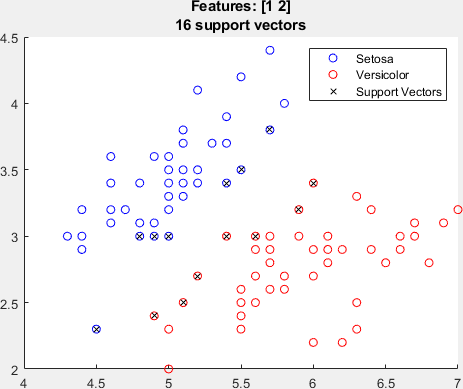
\includegraphics[width = 2in, height = 1.5in]{Q1_6.png}} &
            \subfloat[]{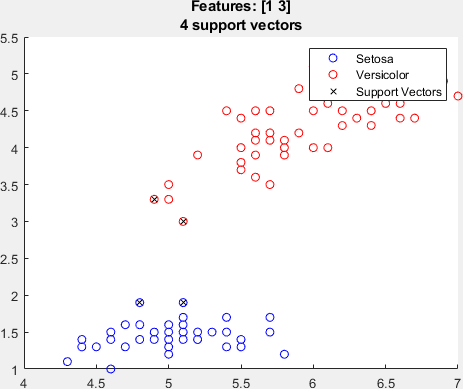
\includegraphics[width = 2in, height = 1.5in]{Q1_5.png}}   \\
            \subfloat[]{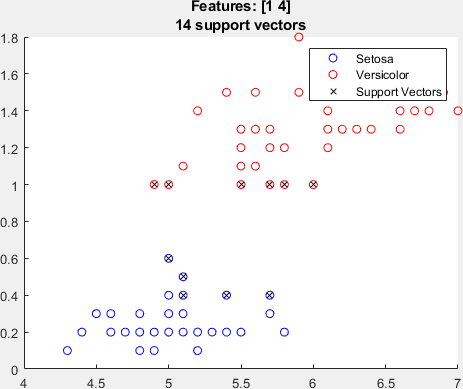
\includegraphics[width = 2in, height = 1.5in]{Q1_4.png}} &
            \subfloat[]{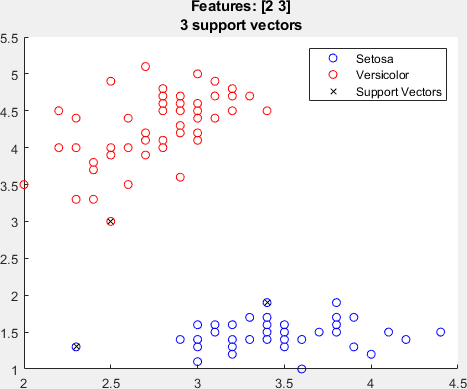
\includegraphics[width = 2in, height = 1.5in]{Q1_3.png}}   \\
            \subfloat[]{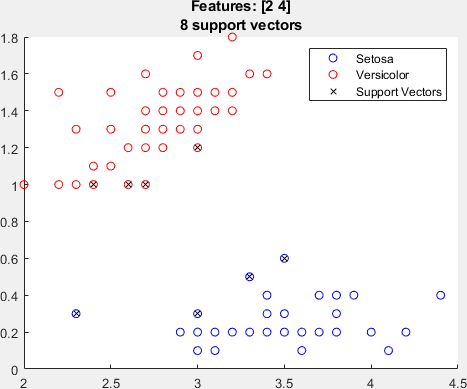
\includegraphics[width = 2in, height = 1.5in]{Q1_2.png}} &
            \subfloat[]{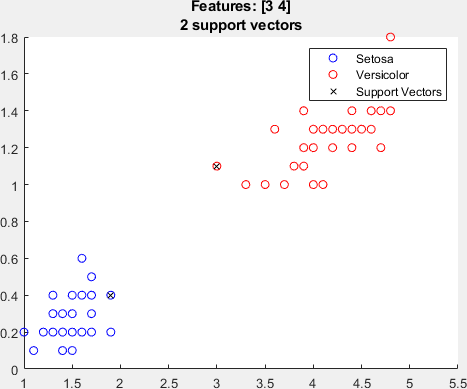
\includegraphics[width = 2in, height = 1.5in]{Q1_1.png}}   \\
        \end{tabular}
        \caption{Support Vectors for different feature pairs}
        \label{fig:q1fig}
    \end{figure}
\end{center}

The number of support vectors was minimum for the features 3 \& 4. One can notice the opposite relationship between the
linear separability of the feature space and the number of support vectors.
However, it is important to note that one can achieve the same number of minimum vectors for other features by setting the
BoxConstraint parameter manually. I observed that setting it to 15 resulted in 2 support vectors for two cases.

\pagebreak

\section{Question 2}

\subsection*{4 Features}
\begin{minipage}{0.3\textwidth}
    $kfold \ loss = 0$
\end{minipage}
\begin{minipage}{0.6\textwidth}
    $LOOCV \ loss = 0$
\end{minipage}
\subsection*{1 Feature}
\begin{minipage}{0.3\textwidth}
    $kfold \ loss = 0.1900$
\end{minipage}
\begin{minipage}{0.6\textwidth}
    $LOOCV \ loss = 0.1700$
\end{minipage}
\vspace*{0.5cm}

Using four features, having higher dimensions, have resulted in SVM Model linearly separating the feature space. Hence,
for both Cross Validation Experiments, the loss rate was 0. On the other hand, when I decreased the number of utilized dimensions
to 1, LOOCV loss was slightly less than the 10-Fold CV loss. This may be attributed to the fact that LOOCV utilizes
more training data than kfold, resulting in higher more accurate test set predictions, considering that the
number of training data is not so large that it causes overfitting.

\pagebreak

\section{Question 3}

\begin{center}
    \begin{figure}[h]
        \begin{tabular}{cc}
            \subfloat[]{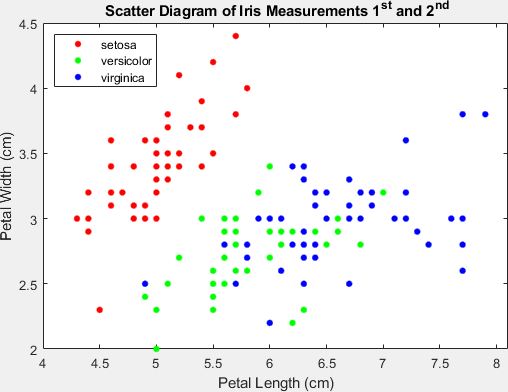
\includegraphics[width = 2in, height = 1.5in]{Q3_4.png}} &
            \subfloat[]{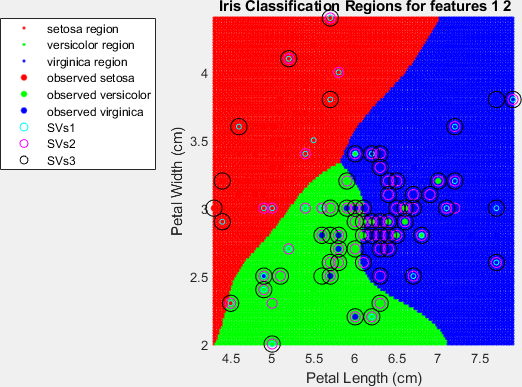
\includegraphics[width = 2in, height = 1.5in]{Q3_3.png}}   \\
            \subfloat[]{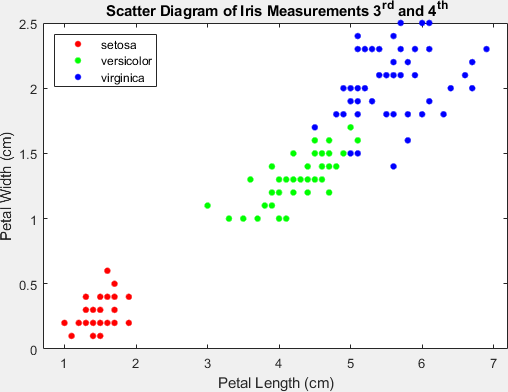
\includegraphics[width = 2in, height = 1.5in]{Q3_2.png}} &
            \subfloat[]{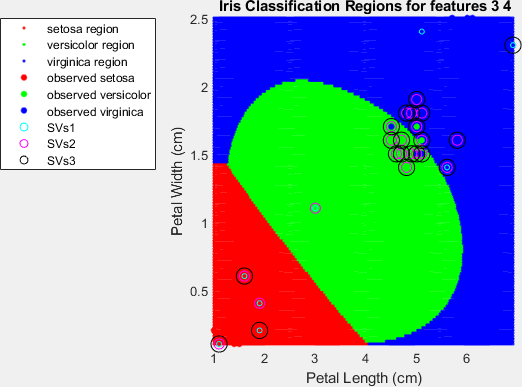
\includegraphics[width = 2in, height = 1.5in]{Q3_1.png}}   \\
        \end{tabular}
        \caption{Support Vectors for different feature pairs}
        \label{fig:q3fig}
    \end{figure}
\end{center}

\vspace*{-1cm}
Changing feature pairs that are utilized in SVM classification resulted in different distributions. Features 3 and 4
provides a more linearly separable feature space than 1 and 2. The resultant numbers of support vectors 196 and 58 also
indicates the same result. In addition, this is also observable in scatter plots.

\section{Question 4}

The objective function, as a function of BoxConstraint and KernelScale, is optimized using Bayesian optimization.
Hence, these parameters determines the cross validation loss and selecting them is a crucial part of optimizing an
SVM classifier, keeping in mind that rbf as kernel function is fixed. In addition, I have tried polynomial kernel
function, and observed that optimized cross validation loss is different from the one that rbf kernel function is
able to achieve. Therefore,
\begin{itemize}
    \item Box Constraint
    \item Kernel Scale
    \item Kernel Function
\end{itemize}
are the hyperparameters that can be optimized in an SVM to achieve better cross validation success, in terms of loss.

\pagebreak
\section{APPENDIX}
The code given in this section is shared \href{https://github.com/kutay-ugurlu/Pattern-Recognition/tree/master/HW3}{@\faGithubSquare}.
\subsection{Q1}\label{subsec:Q1_code}
\lstinputlisting{HW3_Q1.m}
\pagebreak
\subsection{Q2} \label{subsec:Q2_code}
\lstinputlisting{HW3_Q2.m}
\pagebreak
\subsection{Q3}\label{subsec:Q3_code}
\lstinputlisting{HW3_Q3.m}
\pagebreak
\subsection{Q4}\label{subsec:Q4_code}
\lstinputlisting{HW3_Q4.m}
\end{document}